\documentclass{article}

\usepackage{cleveref}
\usepackage{graphicx}
\usepackage{relsize}

\title{%
    Doggochain --- A doggo game blockchain \\
    [0.5em]
    \smaller{2nd report}
}
\author{%
    Guilherme Christopher Michaelsen Cardoso (14100831) \\
    João Paulo Taylor Ienczak Zanette (14200743)
}

\begin{document}
    \maketitle

    \section{Contracts structure}

    This section will only describe contracts briefly just to clarify
    \textbf{what} they are (i.e.\ their role in the system). Further
    explanations of \textbf{how} they behave will be cleared
    in~\Cref{sec:function-desc}.

    In short, the contracts directly related to Doggochain are structured as
    follows:

    \begin{description}
        \item[DoggoChain:] The main contract, hence responsible for managing
            database in respect of Players and Doggos, as well as the
            smart-contract's operations (player challenging, hunting, breeding,
            etc.). Abstracts player's data as an internal \texttt{struct},
            since there's no much use for it outside this contract\footnote{%
                The reason is that the \texttt{Player} structure is needed only
                for players to own their Doggos and mark their existence in the
                block-chain (i.e.\ in the game). Every other operation is done
                considering Doggo-to-Doggo interactions.
            }.
        \item[Doggo:] Works as a simple structure for every Doggo's stats,
            providing an interface that abstract how Doggos evolve (as in stat
            gaining) and what's their real current stats.
        \item[UsageTest:] A unit test to check if the system works properly
            from the point of view of who's going to \textit{use} the API\@.
    \end{description}

    Other implementation-specific contracts are designed to compensate some
    lack of features from Solidity 0.5, e.g.\ no proper dynamic array handling
    in storage data. Currently these contracts are:

    \begin{description}
        \item[DoggoList:] A simple list data structure implementation,
            simulated using a mapping from \texttt{uint32} to \texttt{Doggo}
            (since there's no generics in Solidity, this implementation must be
            replicated for every different type) and a \texttt{length} variable
            for element counting.
        \item[OptionalPlayer:] Actually not a contract itself, but a structure.
            Used to compensate the lack of Optional type\footnote{%
                An ``Optional'' is a type that handles existence/inexistence of
                data (without the security/usage issues of using
                \texttt{null}-like value).
            } in Solidity. Needed since Solidity mappings assume \textit{all}
            possible keys actually exist and maps to some value (meaning no
            \texttt{hasKey}-related checking), and it does not belong directly
            to \texttt{Player} structure since existence itself is not a
            player's property, but rather is a mapping's constraint.
    \end{description}

    Apart from that, there are libraries for the more complex operations, so
    the amount of responsibility in DoggoChain contract's code becomes reduced:

    \begin{description}
        \item[Battle:] For battle simulation. Its only public function is
            \texttt{simulate}, which gives a simulated battle's results.
        \item[Breed:] For breeding operations. Its only public function is
            \texttt{breed}, which gives result containing the (possibly)
            generated Doggo and if the breeding was a success.
    \end{description}


    \section{Function details\label{sec:function-desc}}

    This section will be splitted in a subsection for each \textbf{main
    contract and libraries}, since other contracts are merely for
    implementation details.

    \subsection{DoggoChain}

    \begin{description}
        \item[registerPlayer(string name):] Registers a player in the
            blockchain, making sure the player hasn't been previously
            registered, and initializes their list of Doggos.
        \item[challenge(address target):] Implements the rules for challenging
            a player for a Player versus Player battle.
        \item[breed(Doggo this, Doggo with):] This function implements the
            rules for breeding two Doggos and spawning a new Doggo. The baby
            will have a combination of the hidden attributes of both parents.
        \item[trade(address to, string doggo\_name):] Implements the rules for
            trading a Doggo with a specific player.
        \item[hunt(doggo):] Implements the rules for capturing a wild Doggo and
            adding it to the player's collection.
        \item[player(address addr):] Retruns the name of the player, and their
            list of doggos.
        \item[totalPlayers():] Returns the number of registered players in the
            blockchain.
    \end{description}

    So to use any of the game's features, all the player have to do is to call
    each function from this contract. Each function will require that the
    player is correctly registered and will detect that using the
    \texttt{msg.sender} property as player's address.

    For the \texttt{challenge}, \texttt{trade}, \texttt{breed} and
    \texttt{hunt}, the player will be informed of the \textbf{results} of that
    operation via function return data, with computations updating the storage
    internally. Since they're related to complex actions, some of their
    responsibilities are splitted into other libraries (e.g.\ \texttt{Battle}
    and \texttt{Breed}), so these functions will just call the libraries' ones,
    get the results and take decisions based on them.

    \subsection{DoggoList}

    This is a simple contract that implements a manual array implementation,
    which is necessary because Solidity doesn't implement struct copy from
    memory to storage.

    \begin{description}
        \item[push(Doggo doggo):] Inserts a doggo to the end of the list.
        \item[pop():] Removes and returns the last doggo in the list.
        \item[isEmpty():] Returns true if the list is empty.
    \end{description}

    \subsection{Doggo}

    Aside from the \texttt{DoggoChain} contract (which uses this contract just
    for storing purposes), some code units such as libraries (e.g.\
    \texttt{Battle}) will make extensive use of the \texttt{Doggo} contract's
    functions. To understand how was it modelled, let's see this example:
    during simulation in a battle between two Doggos, called ``first'' and
    ``second'' for reference, the library may want to calculate the results of
    an physical attack action from ``first'' to ``second''. This can be
    achieved by doing the following:

    \begin{enumerate}
        \item The library calls \texttt{first.attack()} and holds its result;
        \item Then, the library calls \texttt{second.defense()} and also holds
            its result;
        \item Since the attack and defense values means, respectively, how much
            physical offensive and defensive power a Doggo has, the library can
            use a formula based on them to calculate a damage value, i.e.\ how
            much ``second'' will suffer with ``first''s attack.
        \item With that damage value calculated, the library will then apply
            that damage into ``second'' calling its own function
            \texttt{damage(target, amount)}, passing \texttt{second} as
            argument to \texttt{target} and the damage value for
            \texttt{amount}.
        \item \texttt{damage(...)} will then decrease the current health points
            (``HP'' for short), i.e.\ how much that doggo can still keep up
            with the battle, which is controlled outside ``Doggo'' contract
            using a separate struct \texttt{Battler} that holds both the
            ``Doggo'' and its current health. This way, battle can be handled
            without ever changing the contract's storage (except when applying
            battle simulation results's side-effects, e.g.\ giving a Doggo its
            experience points --- potentially leveling him up).
    \end{enumerate}

    That should illustrate the idea of this contract's modelling: do as few
    writes as possible to the storage (leaving it only for more ``permanent''
    data) and let the more complex operations built atop the view-only
    functions.

    \section{Diagrams}

    For a more top-level visualization of the contracts's
    schema,~\Cref{fig:class-diagram} shows a Class Diagram for the system as a
    whole, while~\Cref{fig:registerPlayerSD,fig:simulateSD} shows Sequence
    Diagrams for the main complex transactions.

    \begin{figure}[h]
        \centering{}
        \includegraphics[width=1\textwidth]{example-image-a}
        \caption{Class Diagram for DoggoChain system.~\label{fig:class-diagram}}
    \end{figure}

    \begin{figure}[h]
        \centering{}
        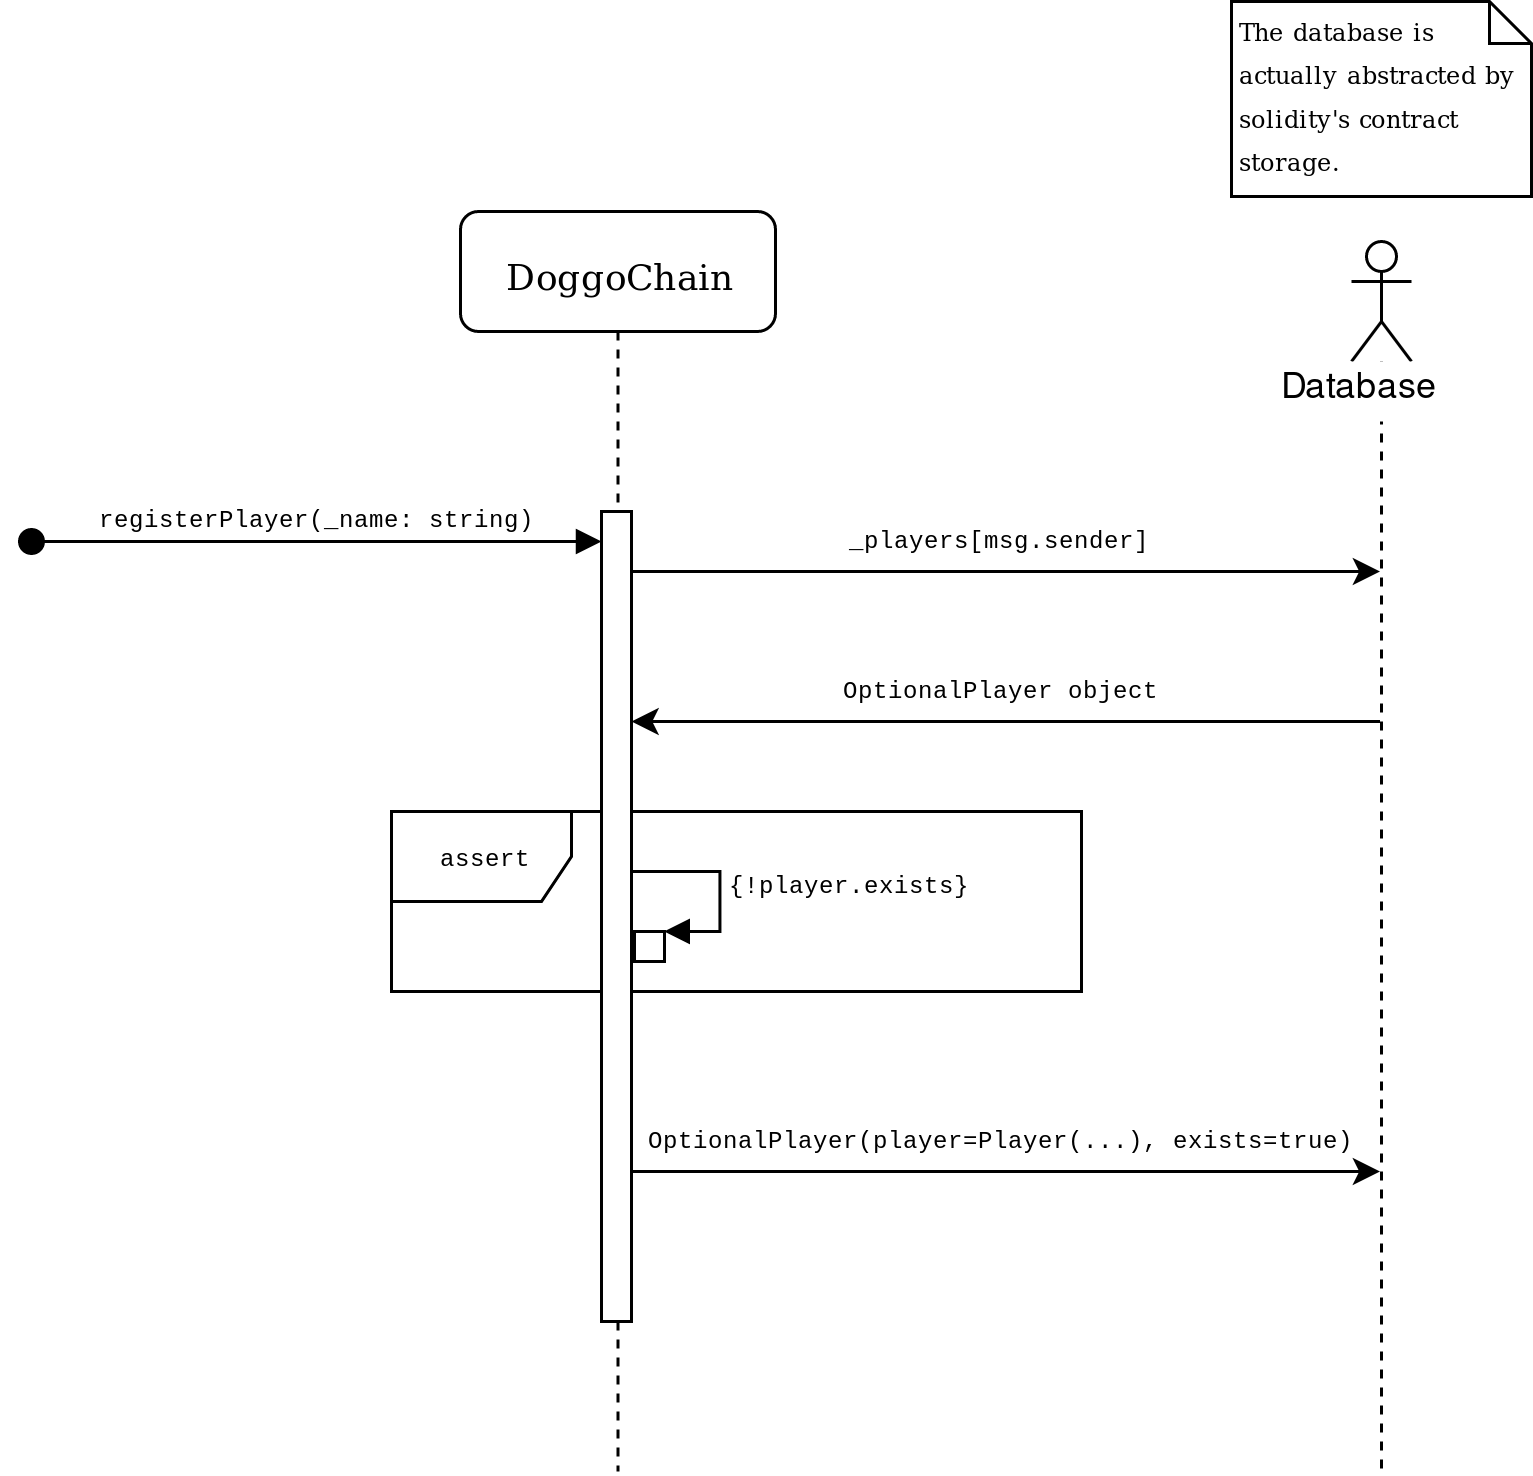
\includegraphics[width=1\textwidth]{img/DoggoChain - registerPlayer SD}
        \caption{%
            Sequence Diagram for \texttt{DoggoChain.registerPlayer}
            function.~\label{fig:registerPlayerSD}
        }
    \end{figure}

    \begin{figure}[h]
        \centering{}
        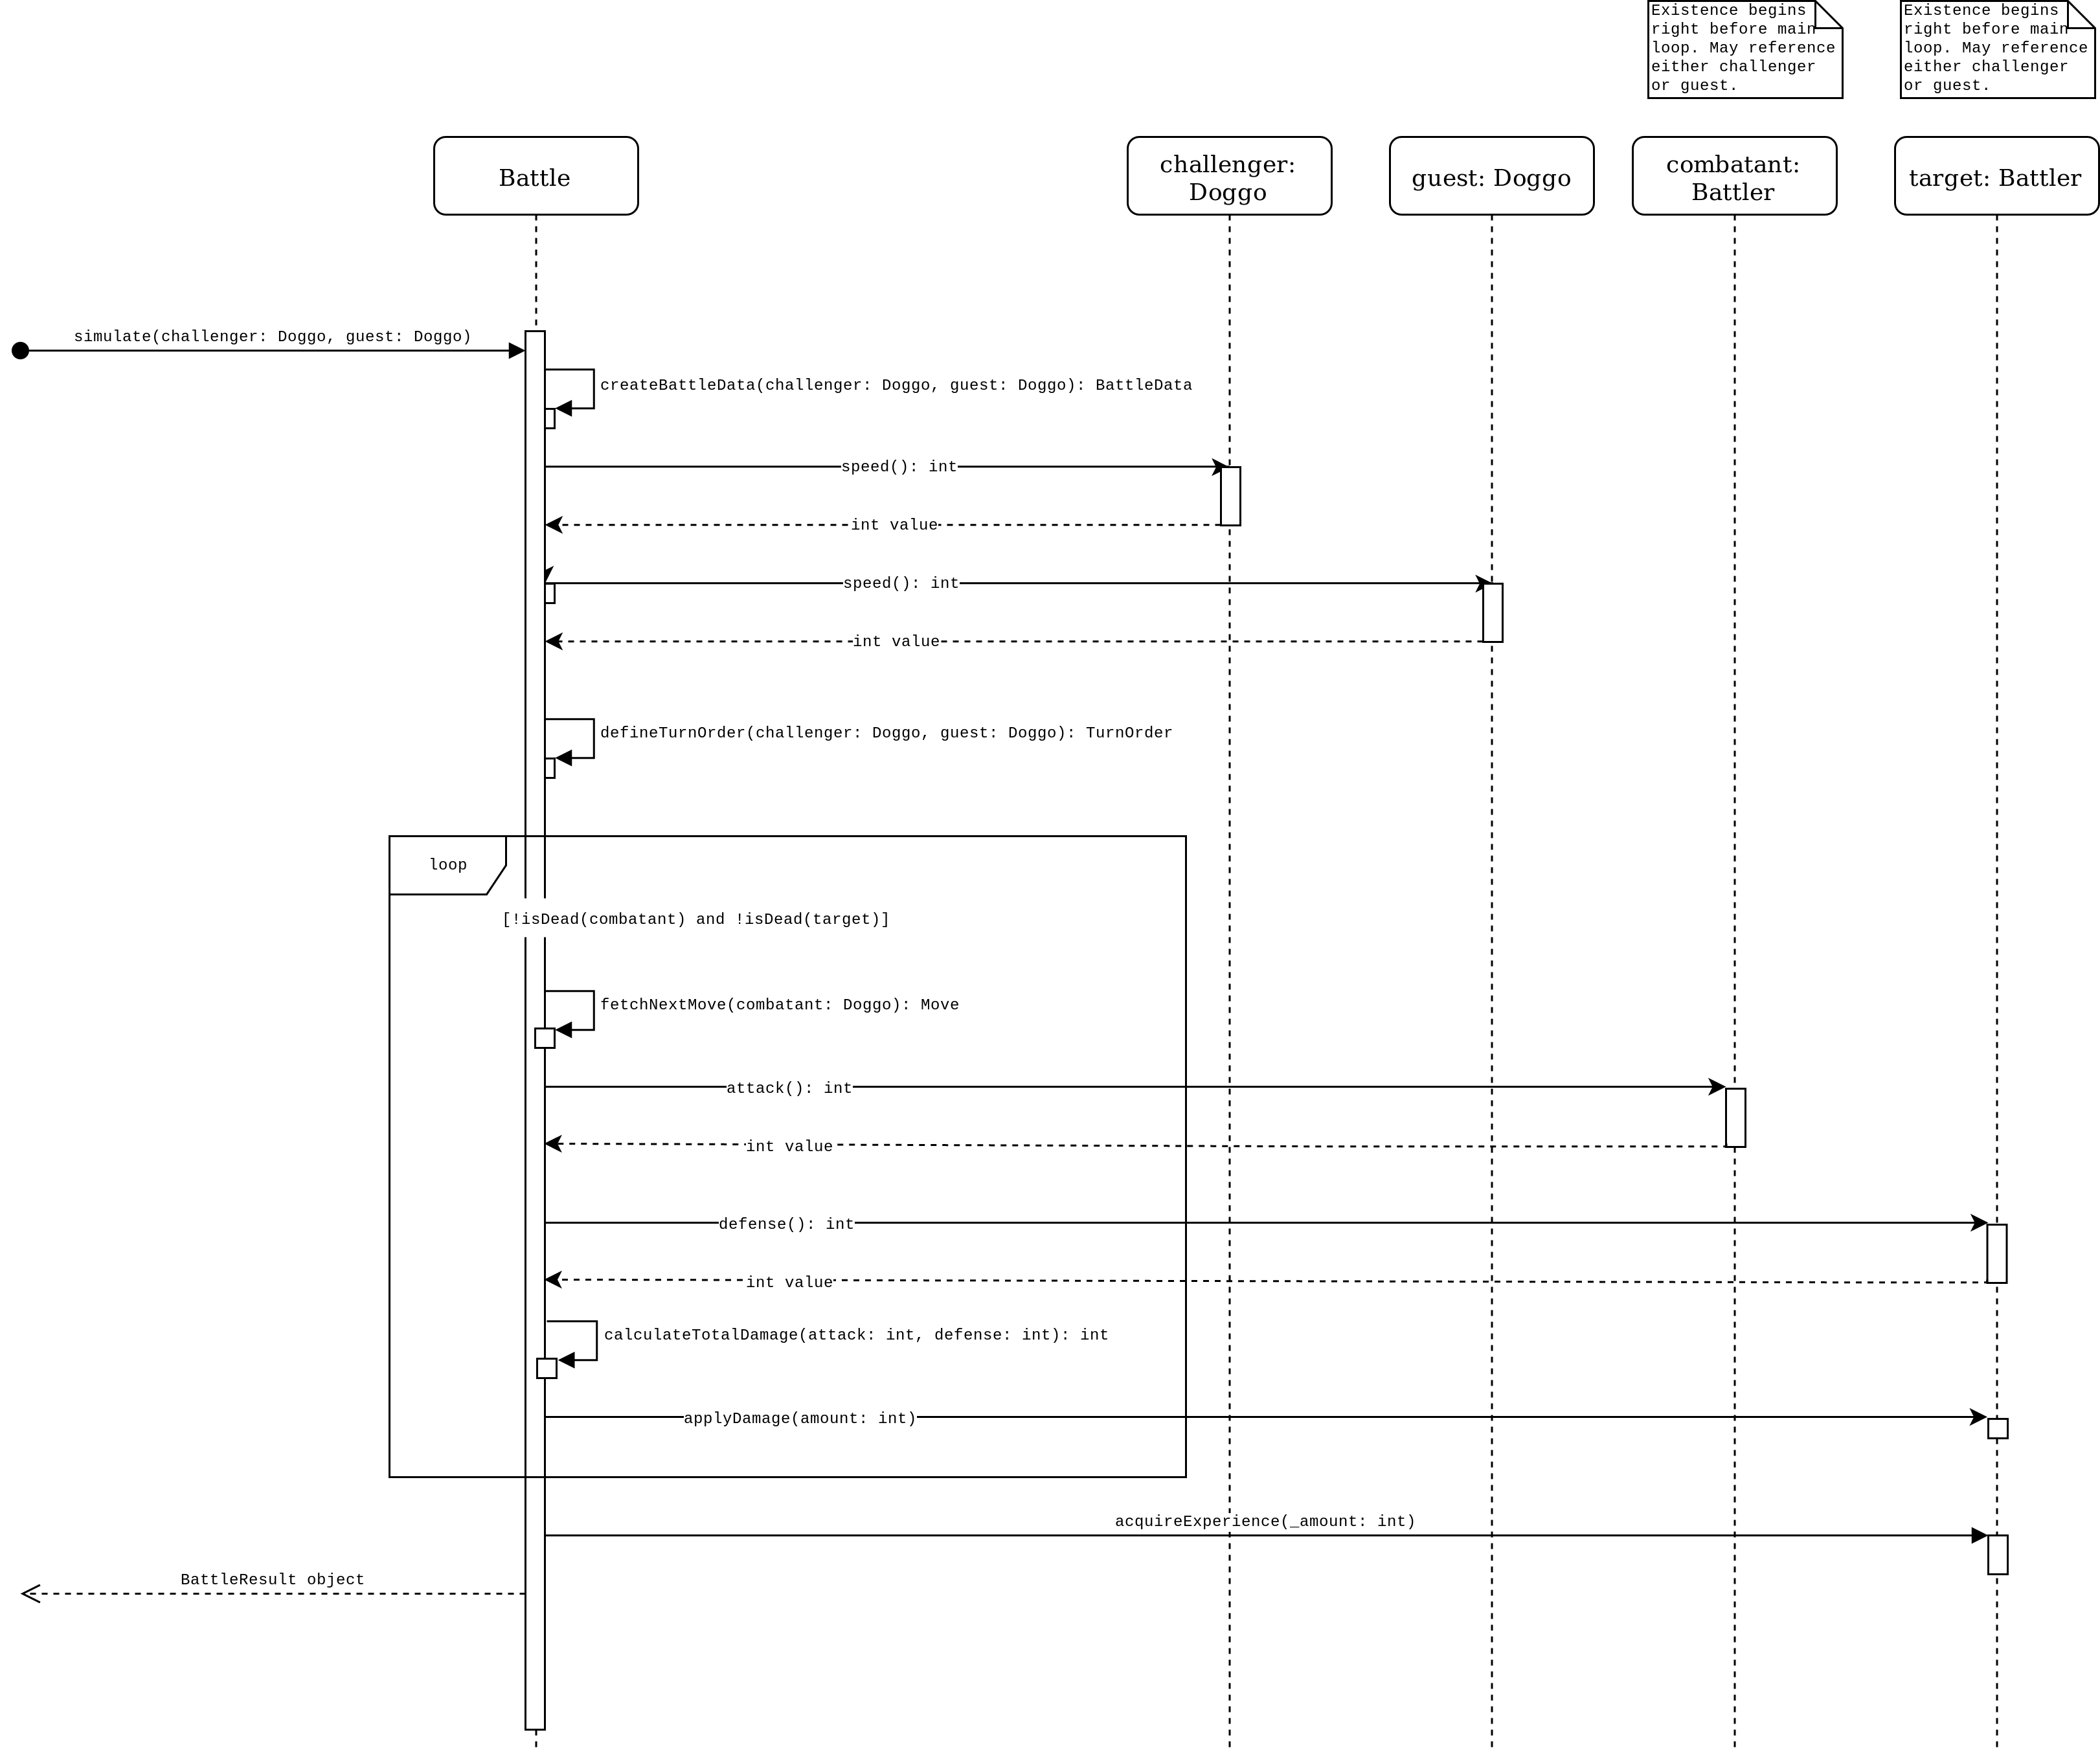
\includegraphics[width=1\textwidth]{img/DoggoChain - simulate SD}
        \caption{%
            Sequence Diagram for \texttt{Battle.simulate}
            function.~\label{fig:simulateSD}
        }
    \end{figure}
\end{document}
